\section{Results}
\label{sec:results}

\begin{equation*}
v_{max}^{np} = \begin{bmatrix}
	0.4025950 \\
	0.4790814 \\
	0.3357358 \\
    0.3835011 \\
    0.3542414 \\
    0.4723555
\end{bmatrix} \quad w_{max}^{np} =  2.83515
\end{equation*}

\begin{equation*}
v_{max}^{nn} = \begin{bmatrix}
	0.4023249 \\
	0.4791663 \\
	0.3364637 \\
	0.3822769 \\
	0.3541386 \\
	0.4730503
\end{bmatrix} \quad w_{max}^{nn} = 2.83514
\end{equation*}

 \begin{figure}[htbp]
 	\centering
 	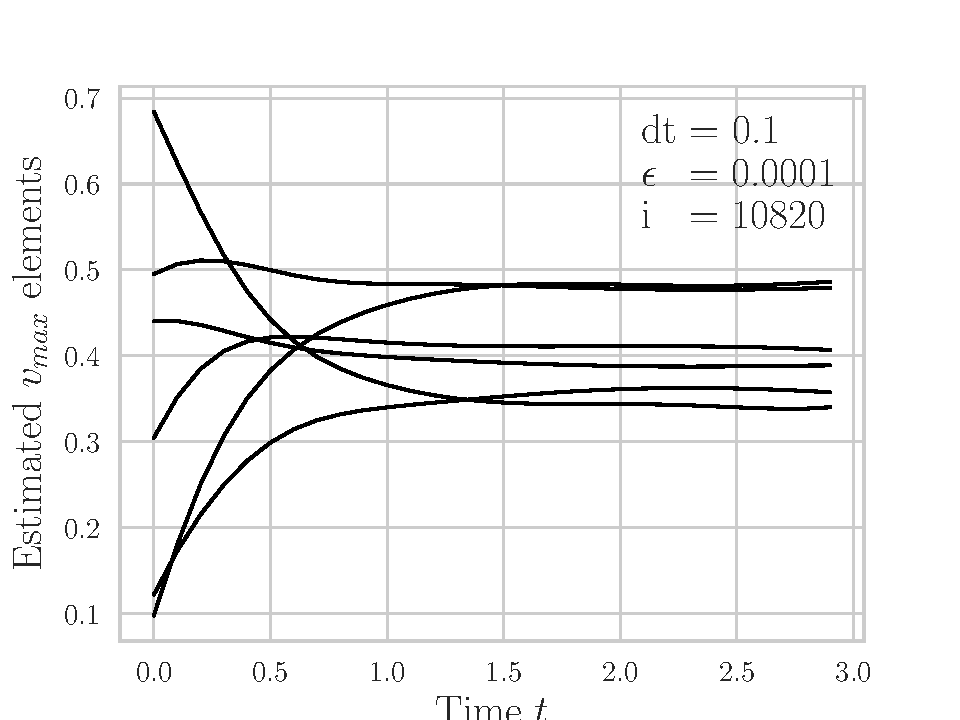
\includegraphics[width=0.5\textwidth]{eigenvector_max}
 	\caption{Figure showing how the value of the elements of the estimated eigenvector $v_{max}$ evolves over time. Each line represents one of the elements of the vector.}
 	\label{fig:eigenvector_max}
 \end{figure}
 
 \begin{equation*}
	 v_{min}^{np} = \begin{bmatrix}
	  0.6928048 \\
	 -0.0074343 \\
	 -0.7048516 \\ 
	 -0.1487365 \\
	 0.0122096 \\
	 0.0296413
	 \end{bmatrix} \quad w_{min}^{np} = -0.515594
 \end{equation*}



 \begin{figure}[htbp]
 	\centering
 	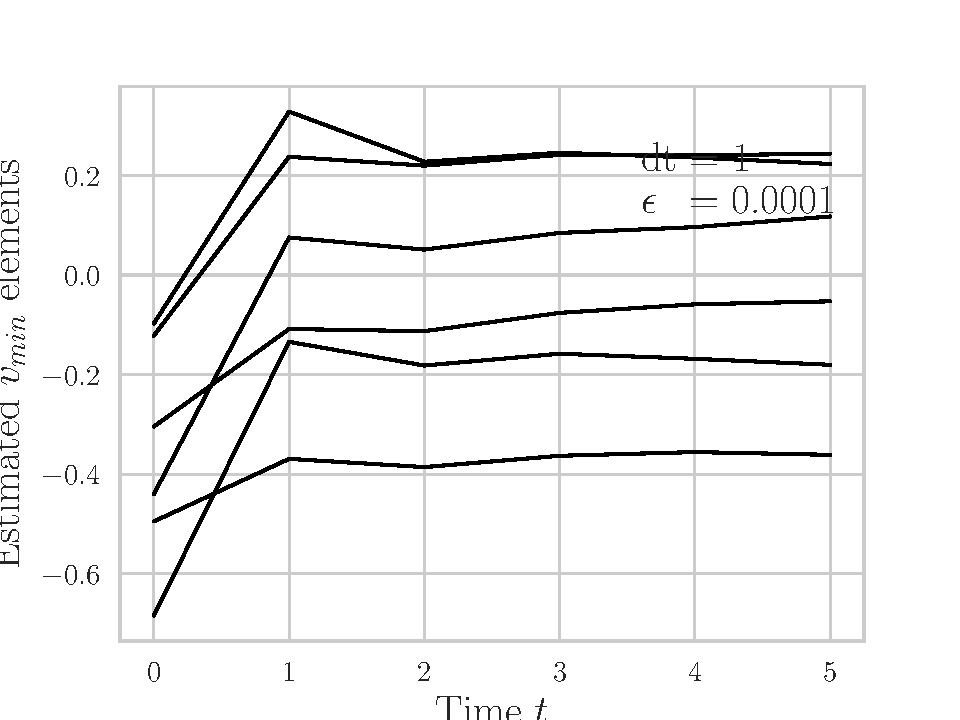
\includegraphics[width=0.5\textwidth]{eigenvector_min}
 	\caption{Figure showing how the value of the elements of the estimated eigenvector $v_{min}$ evolves over time. Each line represents one of the elements of the vector.}
 	\label{fig:eigenvector_min}
 \end{figure}

% Eksempel for figurer
% \begin{figure}[htbp]
% 	\centering
% 	\includegraphics[width=0.5\textwidth]{}
% 	\caption{}
% 	\label{fig:}
% \end{figure}
